\documentclass[a4paper, 12pt, twoside]{report}

\usepackage{physics, amsmath, amsfonts, systeme}
\usepackage{tcolorbox}
\usepackage{enumitem}
\usepackage{hyperref}
\usepackage{graphicx}
\hypersetup{
        colorlinks=true,
                linkcolor=black,
                urlcolor=blue,
}

\usepackage{geometry}
\geometry{
        top=2cm,
                bottom=2cm,
                left=2cm,
                right=3cm,
                headheight=17pt,
                includeheadfoot,
}

\usepackage{fancyhdr, lastpage}
\pagestyle{fancy}
\fancyhf{}
\lhead{Mettere icona GitHub}
\rhead{ Ottica }
\cfoot{Pagina \thepage\ di \pageref{LastPage}}
\renewcommand{\headrulewidth}{1.0pt}

\usepackage{etoolbox}
\patchcmd{\chapter}{\thispagestyle{plain}}{\thispagestyle{fancy}}{}{}

\title{Ottica}
\author{Pietro Garofalo}
\date{\today}


\begin{document}

\maketitle
\newpage
\tableofcontents
\chapter{Gli stati di polarizzazione}
In generale possiamo esprimere la luce come un campo elettrico 
\begin{align*}
    \va{E} = \va{E_{0}}\exp{i(\vb{k}\vb{r}-\omega t + \phi)}
\end{align*}
Il vettore $\va{E}$ è scomponibile in due componenti tra loro sempre ortogonali
\begin{tcolorbox}[colback=red!5!white,colframe=red!50!black,title=ATTENZIONE !]
        se la differenza di fase tra le due componenti $\va{E_{x}}$ ed $\va{E_{y}}$ si mantiene 
        costante si dice che la luce è \textbf{polarizzata}, se invece essa varia nel tempo 
        in modo casuale allora è \textbf{non polarizzata}, es la luce del sole.
\end{tcolorbox}
Semplicemente la polarizzazione ci dice come sono correlate le due componenti del campo elettrico, 
ve ne sono diverse, per esempio prendiamo una luce polarizzata circolarmente:
\begin{figure}[!h]
    \centering
    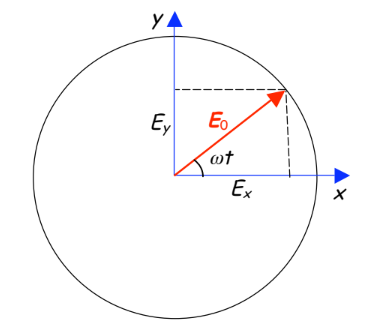
\includegraphics[scale=0.5]{polarizzazione/PolarizzazioneCirc} 
\end{figure}

ossia una luce che ha la compomente x massima quando quella y è nulla. 
\newpage
Possiamo rappresentarla nel seguente modo:
\begin{align*}
    \va{E} = \va{E}_{0x}\cos(kz-\omega t) + \va{E}_{0y}\sin(kz-\omega t)
\end{align*}
passando ora alla notazione complessa :
\begin{align*}
        \va{E} &= \va{E}_{0x}\exp{i(kz-\omega t)} + \va{E}_{0y}\exp{i(kz-\omega t)\pm \frac{\pi}{2}}\\[1em]
               &= \va{E}_{0x}\exp{i(kz-\omega t)} + \va{E}_{0y}i\exp{i(kz-\omega t)}
\end{align*}
dove non ho fatto altro che riscrivere il seno come il coseno più o meno $\frac{\pi}{2}$. \\
\section{Il vettore di Jones}
Dalla formula ricavata prima si nota subito che possiamo riscrivere l'onda come :
\begin{align*}
    \va{E} = \va{E}_{0}\va{J}\exp{i(kz-wt)}
\end{align*}
Dove il vettore $\va{J}$ rappresenta proprio la polarizzazione ed è definito come \textbf{vettore di Jones} che nel caso 
della polarizzazione circolare vale : 
\begin{align*}
        \va{J} = \begin{pmatrix} 1 \\ i \end{pmatrix}
\end{align*}
Tutte le polarizzazioni e i corrispondenti vettori di Jones li allego in figura
\begin{figure}[!h]
    \centering
    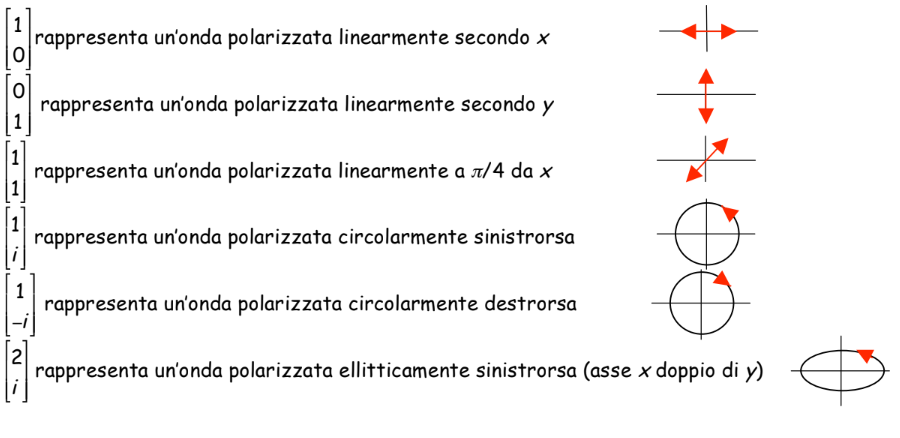
\includegraphics[scale=0.4]{polarizzazione/VettoriJones}
\end{figure}
In quest'ottica dunque gli effetti degli elementi ottici come per esempio le lamine $\lambda/4$ o $\lambda/2$, vengono 
rappresentati come \textbf{matrici di Jones}.
\newpage
\begin{figure}[!h]
    \centering
    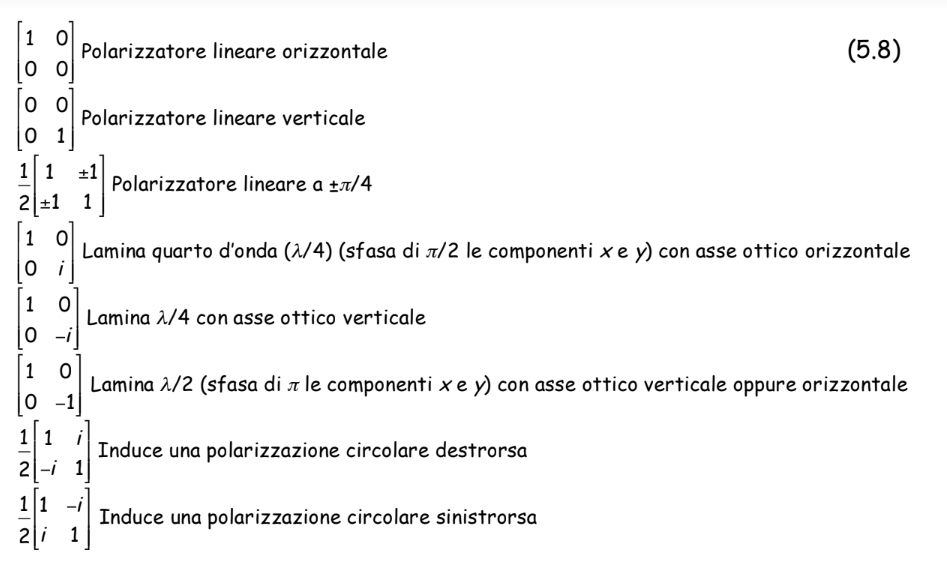
\includegraphics[scale=0.4]{polarizzazione/MatriciJones}
\end{figure}

Facciamo un esempio, prendiamo una luce polarizzata a 45 che passa attraverso una lamina $\lambda/4$:
\begin{align*}
    \begin{pmatrix} 1 & 0 \\ 0 & i\end{pmatrix}\begin{pmatrix}1\\1\end{pmatrix} = \begin{pmatrix}1\\i\end{pmatrix}
\end{align*}
si ottiene una luce polarizzata circolarmente.
Si possono ottenere inoltre gli effetti di altri elementi ottici ruotando quello originale.
Prendendo la matrice di rotazione : 
\begin{align*}
    R(\theta) = \begin{pmatrix}\cos{\theta} & \sin{\theta} \\ -\sin{\theta} & \cos{\theta} \end{pmatrix}
\end{align*}
allora la nuova matrice $\vb{T}^{\prime}$ si ottiene:
\begin{align*}
        \vb{T}^{\prime} = \vb{R}(\theta)\vb{T}\vb{R}(-\theta)
\end{align*}
\begin{tcolorbox}[colback=red!5!white,colframe=red!50!black,title=ATTENZIONE !]
Il fatto che se per esempio prendo un polaroid orizzontale e lo giro di 90 gradi ottendo un polaroid verticale 
funzione perchè gli elementi ottici hanno un asse preferenziale chiamato \textbf{asse ottico}
\end{tcolorbox}

\chapter{Riflessione e rifrazione della luce}
Consideriamo un'onda piana che incide sulla superficie di separazione fra due materiali
che hanno un indice di rifrazione diverso $n_{1}$ ed $n_{2}$, una parte dell'onda incidente 
verrà riflessa ed un altra verrà trasmessa.
\begin{figure}[!h]
    \centering
    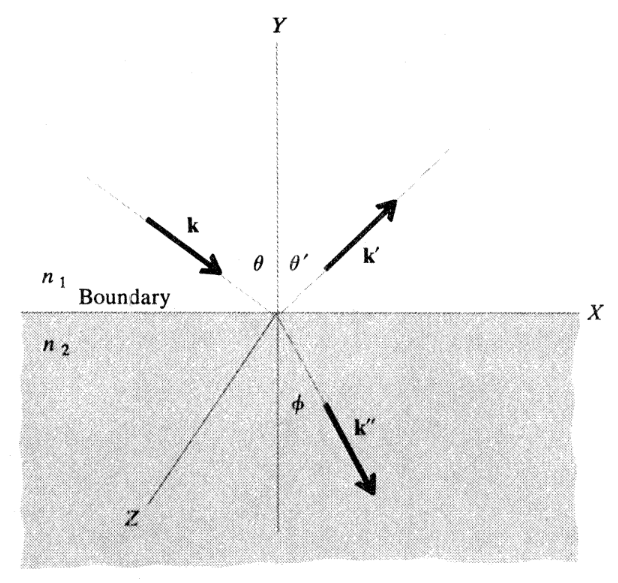
\includegraphics[scale=0.5]{riflessione/Riflessione1}
\end{figure}
Scriviamo la dipendenza spazio-temporale per ciascun'onda :
\begin{align*}
    &\exp{i(\vb{k}\vb{r}-\omega t)} \tag*{Onda incidente}\\
    &\exp{i(\vb{k}^{\prime}\vb{r}^{\prime} - \omega t)}\tag*{Onda riflessa}\\
    &\exp{i(\vb{k}^{\prime\prime}\vb{r}^{\prime\prime}-\omega t)}\tag*{Onda trasmessa}
\end{align*}
Chiamiamo ora \textit{xy} il \textbf{piano di incidenza} e con \textit{xz} il \textbf{piano di interfaccia},
affinchè ci possano essere relazioni costanti è necessario che :
\begin{align*}
    &\omega = \omega^{\prime} = \omega^{\prime\prime} \\
    &\vb{k}\vb{r} = \vb{k}^{\prime}\vb{r}^{\prime} = \vb{k}^{\prime\prime}\vb{r}^{\prime\prime}
\end{align*}
la seconda condizione deve valere sul piano di interfaccia e supponendo che 
la prima onda appartenga al piano di incidenza diventa : 
\begin{align*}
        k_{x}x = k^{\prime}_{x}x + k^{\prime}_{z}z = k^{\prime\prime}_{x}x + k^{\prime\prime}_{z}z 
\end{align*}
ma dovendo valere $\forall{x}$ e $\forall{y}$ allora $k^{\prime}_{y} = k^{\prime\prime}_{y} = 0$
\begin{tcolorbox}[colback=red!5!white,colframe=red!50!black,title=ATTENZIONE !]
        si ottiene che i vettori $\vb{k}$ sono \textbf{complanari}, in particolare che 
        $k_{x} = k^{\prime}_{x} = k^{\prime\prime}_{x}$
\end{tcolorbox}
\section{Legge di Snell}
Scrivendoli ora in funzione della loro lunghezza d'onda
\begin{align*}
    &\lambda = \frac{\lambda_{0}}{n_{1}} \\
    &\lambda^{\prime} = \frac{\lambda_{0}}{n_{1}} \\
    &\lambda^{\prime\prime} = \frac{\lambda_{0}}{n_{2}}
\end{align*}
e ricordando il fatto che sono complanari otteniamo due relazioni fondamentali:
\begin{align*}
    &k_{x} = k^{\prime}_{x} \\
    &\frac{2\pi}{\lambda}\sin{\theta} = \frac{2\pi}{\lambda^{\prime}}sin{\theta^{\prime}}
\end{align*}
\begin{tcolorbox}[colback=red!5!white,colframe=red!50!black,title=ATTENZIONE !]
\begin{align*}
    \theta = \theta^{\prime}
\end{align*}
\end{tcolorbox}
\begin{align*}
    &k_{x} = k^{\prime\prime}_{x} \\
    &\frac{2\pi}{\lambda}\sin{\theta} = \frac{2\pi}{\lambda^{\prime\prime}}sin{\phi}
\end{align*}
\begin{tcolorbox}[colback=red!5!white,colframe=red!50!black,title=ATTENZIONE !]
        \textbf{Legge di Snell}
        \begin{align*}
            n_{1}\sin{\theta} = n_{2}\sin{\phi}
        \end{align*}
\end{tcolorbox}
Possiamo studiare due casi : 
\begin{align*}
    &n_{1}<n_{2} \rightarrow \phi<\theta\\
    &n_{1}>n_{2} \rightarrow \phi>\theta
\end{align*}
In particolare nel secondo caso, all'aumentare di $\theta$ deve quindi aumentare anche $\phi$ 
fino ad arrivare ad un angolo critico ( infatti la funzione seno non può essere $>$ 1 )
\begin{align*}
    \phi_{c} = \frac{\pi}{2}
\end{align*}
in questo caso si ha dunque \textbf{riflessione totale interna }, l'angolo $\theta_{c}$ che 
comporta tale situazione è dato dalla legge di Snell:
\begin{align*}
    \theta_{c} = \sin^{-1}{\frac{n_{2}}{n_{1}}}
\end{align*}
\section{Ampiezza delle onde trasmesse e riflesse}
Supponiamo di avere un'onda elettromagnetica che incide sul piano, come sappiamo il campo 
elettrico e quello magnetico sono, in ogni momento, perpendicolari fra loro.
Ricordando le relazioni di continuità :
\begin{align*}
    &E_{1t} = E_{2t}  & D_{1n}=D_{1n}
\end{align*}
valide per mezzi trasparenti ed in assenza di cariche e correnti, possiamo ricavare i coefficienti di 
riflessione e trasmissione. 
Conviene dividire la trattazione in due casi.
\newpage
\subsection{Onda T.M.}
Indichiamo con onda T.M. l'onda che arriva con il campo magnetico \textbf{parallelo} al piano 
di interfaccia \textit{xz} ( transverse magnetic ), dalla figura iniziale quindi uscente dal foglio
mentre il campo magnetico appartiene al piano \textit{xy}
\begin{figure}[!h]
    \centering
    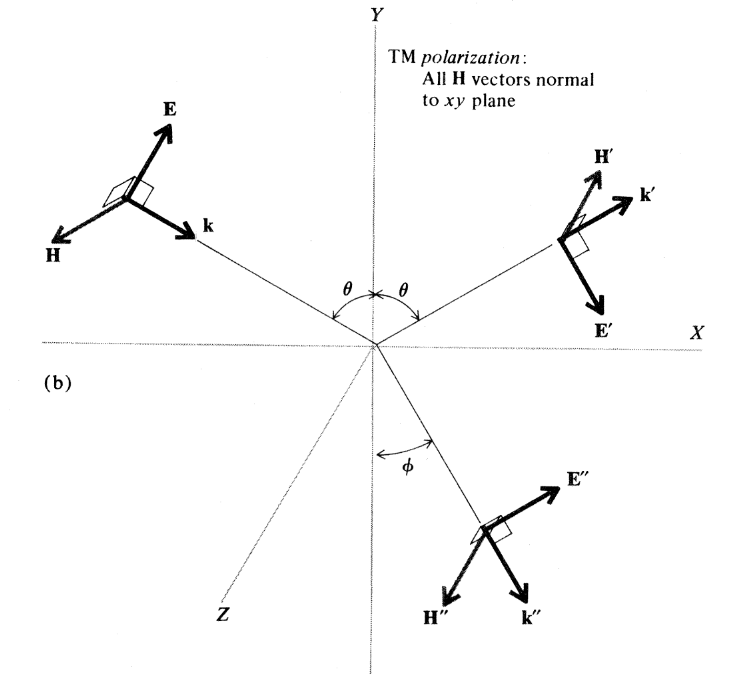
\includegraphics[scale=0.3]{riflessione/OndaTM}
\end{figure}

Le condizioni di continuità si possono scrivere come ( indichiamo $\cos{\theta}$ C e $\sin{\theta}$ S ):
\begin{align*}
    &A) EC - E^{\prime}C = E^{\prime\prime}C^{\prime\prime}\\
    &B) n^2_{1}(ES + E^{\prime}S) = n^2_{2}E^{\prime\prime}S^{\prime\prime}
\end{align*}
ricavando dalla B) $E^{\prime\prime}$ e ricordandoci la legge di Snell $n^2_{1}/n^2_{2}=S^{\prime\prime}/S$, non faccio i calcoli ma sono banali, 
possiamo ricavare \textbf{l'idice di rifrazione} $r_{p}$:
\begin{align*}
        r_{p} = \frac{E^{\prime}}{E} &= \frac{CS-C^{\prime\prime}S^{\prime\prime}}{CS+C^{\prime\prime}S^{\prime\prime}}\\[1em]
                                     &= -\frac{\tan{\theta-\theta^{\prime\prime}}}{\tan{\theta+\theta^{\prime\prime}}}
\end{align*}
Con pochi semplici calcoli si può trovare pure \textbf{l'indice di trasmissione} $t_{p}$ : 
\begin{align*}
    t_{p} = \frac{E^{\prime\prime}}{E} = \frac{2SC^{\prime\prime}}{\sin{\theta+\theta^{\prime\prime}}\cos{\theta-\theta^{\prime\prime}}}
\end{align*}
\newpage
\subsection{Onda T.E.}
L'onda T.E. è quella che arriva con il campo elettrico parallelo al piano di interfaccia \textit{xz}.
\begin{figure}[!h]
    \centering
    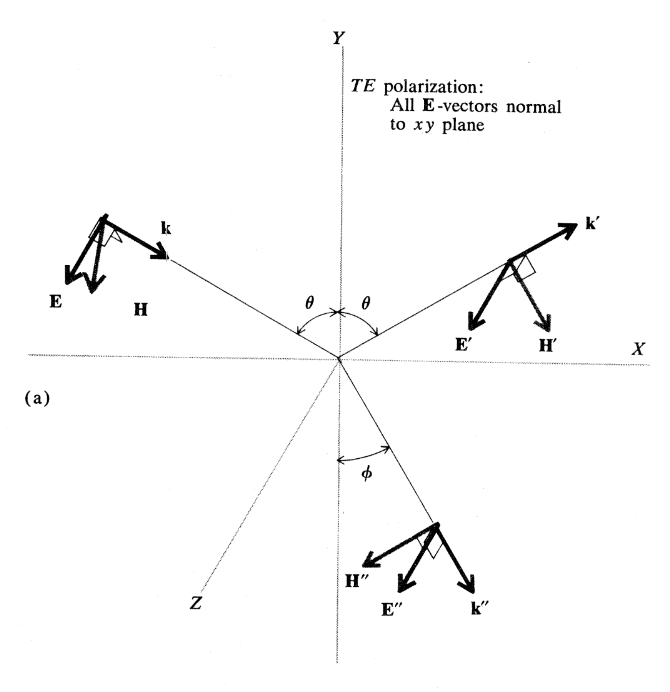
\includegraphics[scale=0.4]{riflessione/OndaTE}
\end{figure}
Applicando le stesse condizioni di continuità si ottiene : 
\begin{align*}
    &r_{s} = -\frac{\sin{\theta-\theta^{\prime\prime}}}{\sin{\theta+\theta^{\prime\prime}}} \\[1em]
    &t_{p} = 1-r_{p}
\end{align*}
\begin{tcolorbox}[colback=red!5!white,colframe=red!50!black,title=ATTENZIONE !]
        Le equazioni degli indici di riflessione e trasmissione sono dette \\ \textbf{relazioni di Fresnel}
\end{tcolorbox}
\newpage
\subsection{Studio degli indici di rifrazione}
L'andamento degli indici di rifrazione è dato dai seguenti grafici che variano nel caso in cui $n_{1}/n_{2}$ sia maggiore o minore di 1: 
\begin{figure}[!h]
    \centering
    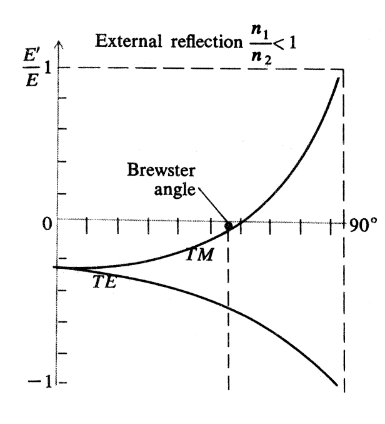
\includegraphics[scale=0.5]{riflessione/R1}
\end{figure}
\begin{figure}[!h]
    \centering
    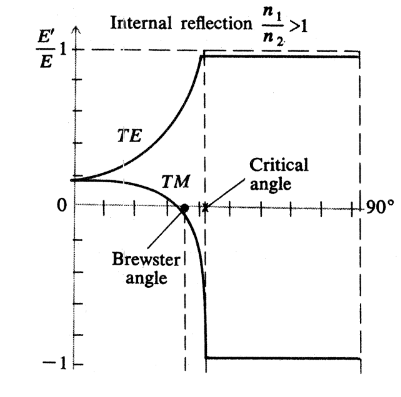
\includegraphics[scale=0.5]{riflessione/R2}
\end{figure}
La prima cosa che notiamo è quando $\theta=0$ che è il caso denominato \textbf{Incidenza normale},
in questo caso 
\begin{align*}
    r_{s} = r_{p} = \frac{n_{1}-n_{2}}{n_{1}+n_{2}}
\end{align*}
in tale contesto $r \approx 1/5$, il segno ovviamente dipende dal fatto se $n_{1}>n_{2}$ 
o viceversa.
\newpage
un'altra cosa da notare è il fatto che $r_{p}$ può essere 0, questo è dato dal fatto che 
\begin{align*}
    r_{p} = \frac{\tan{\theta-\theta^{\prime\prime}}}{\tan{\theta+\theta^{\prime\prime}}}
\end{align*}
si può avere il caso in cui :
\begin{align*}
    &\theta+\theta^{\prime\prime} = \frac{\pi}{2} \Longrightarrow \tan{\theta+\theta^{\prime\prime}}\rightarrow\inf\\
    &r_{p}\rightarrow0
\end{align*}
tale angolo è denominato \textbf{Angolo di Brewster} $\theta_{b}$ che si ottiene grazie alla legge di Snell
\begin{align*}
    &n_{1}\sin{\theta} = n_{2}\sin{\theta^{\prime\prime}}\\
    &n_{1}\sin{\theta} = n_{2}\sin{\frac{\pi}{2}-\theta} \tag*{$\theta+\theta^{\prime\prime} = \frac{\pi}{2}$}\\
    &\tan{\theta_{b}} = \frac{n_{2}}{n_{1}}
\end{align*}
Un'altra cosa da notare nel grafico è che nel caso $\frac{n_{1}}{n_{2}}>1$ i coefficienti di riglessione
hanno una forte risalita in coincidenza di quello che è l'angolo limite visto prima.

\end{document}

